%%
%% Copyright 2019-2024 Elsevier Ltd
%%
%% Version 2.4
%%
%% This file is part of the 'CAS Bundle'.
%% --------------------------------------
%%
%% It may be distributed under the conditions of the LaTeX Project Public
%% License, either version 1.2 of this license or (at your option) any
%% later version.  The latest version of this license is in
%%    http://www.latex-project.org/lppl.txt
%% and version 1.2 or later is part of all distributions of LaTeX
%% version 1999/12/01 or later.
%%
%% The list of all files belonging to the 'CAS Bundle' is
%% given in the file `manifest.txt'.
%%
%% Template article for cas-dc documentclass for
%% double column output.

%\documentclass[a4paper,fleqn,longmktitle]{cas-dc}
\documentclass[a4paper,fleqn]{cas-sc}

%\usepackage[authoryear,longnamesfirst]{natbib}
%\usepackage[authoryear]{natbib}
\usepackage[numbers]{natbib}
\usepackage{cleveref}
\usepackage{pgfplots}
\pgfplotsset{compat=1.18}

\crefname{figure}{Fig.}{Figs.}
\crefname{equation}{Eq.}{Eqs.}
\crefname{table}{Table}{Tables}
\renewcommand{\figurename}{Fig.}
%%%Author definitions
\def\tsc#1{\csdef{#1}{\textsc{\lowercase{#1}}\xspace}}
\tsc{WGM}
\tsc{QE}
\tsc{EP}
\tsc{PMS}
\tsc{BEC}
\tsc{DE}
%%%
\graphicspath{{../IEEE-Transactions-LaTeX2e-templates-and-instructions/}}

\begin{document}
\let\WriteBookmarks\relax
\def\floatpagepagefraction{1}
\def\textpagefraction{.001}
\shorttitle{PointSS}
\shortauthors{Wang and Zhang}

\title [mode = title]{PointSS: Geometry-Aware Multi-Scale State Space Feature Learning for Point Clouds}
\author[1,2,3]{Xin Wang}[orcid=0000-0003-1537-2731]
\cormark[1]
\ead{w_x@jlu.edu.cn}
\author[1]{Xinyuan Zhang}[orcid=0009-0006-4933-1216]

\affiliation[1]{organization={School of Software, Jilin University},
  city={Changchun},
  country={China}}
\affiliation[2]{organization={School of Computer Science and Technology, Jilin University},
  city={Changchun},
  country={China}}
\affiliation[3]{organization={Key Laboratory of Symbolic Computation and Knowledge Engineering of Ministry of Education, Jilin University},
  city={Changchun},
  country={China}}
\cortext[1]{Corresponding author}

\begin{abstract}
State Space Models (SSMs) offer linear computational complexity for point cloud analysis but suffer from spatial proximity loss when serializing 3D point clouds into 1D sequences. To address this limitation, we propose PointSS, a geometry-aware multi-scale state space framework. We introduce a Global Geometry-Aware Mechanism (GGAM) that injects explicit geometric priors through fully connected local graphs constructed within serialization windows on dual orderings (Z-order and Hilbert curves). Edge features encoding surface normals, curvature, and angular deviations are extracted and aggregated via cross-sequence attention and gated fusion to compensate for the loss of spatial proximity. Building on these geometric priors, we design an Adaptive Scale-Decoupled State Space Model (ASD-SSM) that implements a dynamic parameter generation mechanism: the state transition parameter $\bar{A}$ adapts to local geometric characteristics via input-dependent generation, while scale constraint factors remain fixed across scales to control state decay rates hierarchically. On S3DIS Area 5, PointSS achieves 73.8\% mIoU, outperforming Point Transformer V3 (73.4\%) and SSM-based methods including Pamba (73.5\%) and Point Cloud Mamba (69.8\%). On ModelNet40, it achieves 94.6\% overall accuracy. Compared to Point Transformer V3, PointSS achieves 9--19\% faster inference while maintaining linear complexity.
\end{abstract}


\begin{keywords}
Geometry-Aware Feature Learning \sep Multi-Scale Representation \sep Point Cloud Serialization \sep Point Cloud Analysis \sep State Space Models
\end{keywords}

\maketitle



\section{Introduction}
Point clouds serve as a primary representation for 3D scene understanding but present challenges for feature extraction owing to their sparse and unstructured nature. Pioneering works such as PointNet and PointNet++ \cite{pointnet,PointNet++} established efficient point-wise processing paradigms. Despite their efficiency, their limited ability to capture local structures often leads to sub-optimal prediction accuracy. To address this limitation, Transformers \cite{attention,pt,ptv2,ptv3} subsequently improved semantic representation via self-attention; however, their quadratic complexity $\mathcal{O}(N^2)$ creates scalability bottlenecks.

Recently, State Space Models (SSMs) \cite{ssm,Mamba,VisionMamba}, exemplified by
PointMamba \cite{PointMamba} and PCM \cite{pcm}, have gained attention
due to their linear complexity. However, serializing 3D point clouds into
1D sequences will inevitably sacrifice spatial proximity. As illustrated on the left side of \cref{fig:analysis}, some neighboring points can be far apart
after serialization---points that are spatially close may become
distant in the sequence. Such a loss of
proximity is difficult to mitigate in Mamba's recurrent mechanism:
as spatially adjacent points often fall far apart after serialization,
information between them decays before reaching each other's states,
preventing the model from effectively capturing local geometric
structures such as surface normals and curvature. This issue is
particularly pronounced at object boundaries (e.g., wall-pillar
junctions), where accurate segmentation depends critically on
interactions between spatially proximate points that are far apart
after serialization.

\begin{figure*}
	\centering
	\includegraphics[width=.9\textwidth]{picture/analysis.JPG}
	\caption{Identification of the spatial proximity loss problem in existing SSMs (e.g., PCM) and our proposed PointSS solution.}
	\label{fig:analysis}
\end{figure*}
Existing SSM-based methods struggle to establish effective hierarchical representations. Single-scale models (e.g., PointMamba) adopt a non-hierarchical architecture, limiting their ability to simultaneously capture fine-grained geometric details and coarse-scale semantic context.

Hierarchical approaches (e.g., PCM) allocate separate parameters for each downsampled scale. However, their state transition parameters remain input-invariant across spatial locations. This means the network applies identical feature aggregation rules across an entire scale, failing to adapt to varying local geometric characteristics---for instance, processing flat surfaces and sharp boundaries with the same transition dynamics. Furthermore, allocating independent parameters for every scale introduces parameter growth and memory overhead. Consequently, the lack of dynamic, geometry-aware parameterization limits the capacity of existing SSMs to accurately model complex 3D scenes.


To address these limitations, we propose PointSS, a geometry-aware multi-scale state space framework. As depicted in the middle of \cref{fig:analysis}, PointSS explicitly injects geometric priors to alleviate the loss of spatial proximity. Leveraging these geometric priors, we introduce an adaptive multi-scale learning mechanism with scale-decoupled parameterization. Fine scales maintain small state transition parameters for rapid state decay to capture local geometric detail, while coarse scales maintain large values for slow decay to model long-range global context. As shown on the right side of \cref{fig:analysis}, this design enables PointSS to respond more effectively to local geometric variations, producing sharper, more accurate boundaries compared to other SSM methods.

The main contributions of this work are as follows:

\begin{enumerate}
	\item We propose a Global Geometry-Aware Mechanism (GGAM) that injects
	explicit geometric priors through windowed neighborhoods and dual-
	serialization fusion, effectively mitigating the loss of spatial proximity
	and providing reliable geometric guidance for scale-adaptive learning.

	\item We design an Adaptive Scale-Decoupled State Space Model (ASD-SSM)
	featuring a dynamic parameter generation mechanism. By adapting state
	transition parameters $\bar{A}$ to local geometric characteristics, ASD-SSM
	enables fine scales to capture geometric details while coarse scales model
	semantic context, achieving effective hierarchical representations.

	\item Extensive experiments demonstrate that PointSS achieves 73.8\% mIoU
	on S3DIS semantic segmentation and 94.6\% OA on ModelNet40 classification,
	consistently outperforming major SSM-based counterparts while maintaining linear complexity.
	Comprehensive ablation studies further validate the effectiveness of our
	geometry-aware multi-scale design.
\end{enumerate}

Code will be released at https://github.com/z1xy2/PointSS-public.git


\section{Related Work}
\subsection{Deep Learning-based Point Cloud Semantic Analysis}
PointNet \cite{pointnet} pioneers handling the unordered nature of point clouds via symmetric functions. To overcome its limited capacity for local detail modeling, PointNet++ \cite{PointNet++} introduces hierarchical sampling. Subsequent works like DGCNN \cite{DGCNN} enhance local feature modeling via dynamic graph construction. KPConv~\cite{KPConv} generalizes convolution to point clouds through kernel point operators, while PAConv~\cite{paconv} and CurveNet~\cite{curvenet} further advance local feature learning via position-adaptive kernels and curve-based aggregation. PointMLP~\cite{pointmlp} revisits network design by building an effective residual MLP framework with geometric affine modules. However, these convolution-based methods remain constrained by limited receptive fields, limiting effective hierarchical feature construction.

Transformers enable effective global context modeling by leveraging self-attention mechanisms. PCT~\cite{PCT} applies a global attention mechanism specifically designed for point cloud analysis. Point Transformer \cite{pt} integrates positional encoding for spatial awareness, while Stratified Transformer~\cite{stratified_transformer} and Fast Point Transformer~\cite{fast_point_transformer} improve hierarchical and efficient processing. PTv3 \cite{ptv3} achieves state-of-the-art performance using simplified serialization methods. Pre-training strategies such as masked autoencoders~\cite{pointmae} and BERT-style self-supervised learning~\cite{Point-BERT} have further improved Transformer-based point cloud representations. Despite their advantages, the quadratic complexity $\mathcal{O}(N^2)$ creates bottlenecks for large-scale processing. This forces these models to rely on coarse-grained representations, inherently compromising fine-grained local geometric
details.

State Space Models (SSMs) \cite{Mamba} offer a promising alternative with linear complexity. Methods like PointMamba \cite{PointMamba} and PCM \cite{pcm} adapt SSMs by serializing 3D clouds into 1D sequences.   However, this adaptation introduces two key challenges. First,
serialization methods disrupt the spatial relationships between
neighboring points critical for local geometric structure, resulting in
the loss of spatial proximity. Second, uniform serialization struggles to
capture both fine-grained local features and long-range contextual
dependencies, limiting its ability to handle multi-scale representations.


\subsection{Point Cloud Analysis via Geometric Feature Enhancement}

Explicit modeling of geometric attributes, such as surface normals and
curvature, is critical for accurate 3D structural understanding. To
incorporate geometric priors, PointGA \cite{pointga} employs
trigonometric positional encoding to expand raw 3D coordinates
into enriched geometric features. Similarly, PointMSGT \cite{pointmsgt}
utilizes a multi-scale framework with a Geometric Feature Extraction
(GFE) module to reconstruct local triangular structures for detailed
relationship modeling. Geo-CNN \cite{geo-cnn} further captures
structural dependencies via basis decomposition and distance-weighted
aggregation. RepSurf~\cite{repsurf} represents local surfaces via geometric primitives to enhance structural understanding. PointVector~\cite{pointvector} introduces vector-based representations to capture directional geometric information. Spectral-domain approaches such as PointWavelet~\cite{pointwavelet} analyze point cloud structure in the frequency domain for more expressive feature learning. Graph-based methods including dual-graph attention convolution~\cite{dgacn} and local-global graph convolution~\cite{lggcm} exploit both local and non-local geometric dependencies. Works on LiDAR-based segmentation~\cite{lidar_segmentation} further highlight the importance of structured geometric reasoning in large-scale scenes. However, effectively integrating explicit geometric priors
with learned deep features while maintaining computational efficiency
remains a significant challenge.


\subsection{Multi-Scale Representation in Point Cloud Analysis}

Multi-scale feature fusion has been widely adopted in point cloud analysis since PointNet++\cite{PointNet++}, which introduced hierarchical set abstraction
layers for progressive downsampling and local feature aggregation. PointNeXt~\cite{pointnext} revisits PointNet++ with improved training and scaling strategies, demonstrating that architectural improvements at the data pipeline level can yield substantial gains. Subsequent
works have explored various fusion strategies: Transformer-
based methods such as PTv2 \cite{ptv2} and PTv3 \cite{ptv3} adopt U-Net
architectures with hierarchical attention mechanisms. OctFormer~\cite{octformer2} extends octree structures for efficient multi-scale point cloud modeling. CCMNet~\cite{ccmnet} explores multi-scale and cross-type feature interactions for improved 3D learning. RandLA-Net~\cite{Randla} demonstrates that random sampling with a local feature aggregation module enables effective processing of large-scale scenes. These approaches
demonstrate the importance of  multi-scale modeling.

Recent SSM-based methods have attempted to bring linear complexity to point
cloud analysis. PointMamba \cite{PointMamba} employs a plain, non-hierarchical
Mamba backbone, utilizing space-filling curves (Z-order and Hilbert) for
serialization. This design prioritizes
simplicity and efficient modeling of global dependencies but processes all points at a single
feature granularity, lacking the explicit hierarchical structure proven
effective by prior works. In contrast, PCM \cite{pcm} introduces hierarchical
downsampling to capture multi-scale features. While this addresses PointMamba's
single-scale limitation, PCM allocates separate parameter sets for each scale,
with the state transition parameters remaining input-invariant across all
spatial locations within each scale. Consequently, the model applies identical
state transitions to all points—processing flat surfaces and sharp boundaries
with the same transition dynamics—preventing adaptation to local geometric
variations. Furthermore, allocating independent parameters for each scale
incurs parameter growth and memory overhead.
These limitations motivate the design of PointSS, which we describe in detail in the following section.


\section{Method}

\subsection{Framework Overview}

The overall architecture of the PointSS model is illustrated in \cref{fig:architecture}. After data augmentation, the point cloud is serialized into a 1D sequence\cite{ptv3}. We then employ the Global Geometry-Aware Mechanism (GGAM) to extract explicit geometric priors from the serialized sequence. The feature learning component adopts a U-shaped encoder-decoder architecture. To ensure each patch contains an equal number of points, some points may appear in multiple patches (highlighted in orange). The learned features are subsequently fed into a prediction head to produce the final segmentation or classification results. Compared to PCM, this scheme performs serialization only once at the beginning, enabling downsampling via pooling on the serialized point cloud rather than performing re-serialization at each downsampling stage, thereby avoiding the repeated $\mathcal{O}(N\log N)$ serialization overhead.

\cref{fig:coder} illustrates the encoder architecture. ASD-SSM is integrated into both the encoder and decoder for hierarchical feature learning. The decoder adopts a structure symmetric to that of the encoder but replaces pooling with upsampling. Through skip connections from encoder stages, the decoder integrates multi-scale features during the upsampling process.

\begin{figure}
	\centering
	\includegraphics[width=.9\columnwidth]{picture/architecture.jpg}
	\caption{The overview of the proposed PointSS. The encoder and decoder employ a patch-based strategy for point cloud upsampling and down-sampling. The notation (number of points, feature dimension) in Feature Learning indicates the tensor shape at each stage.}
	\label{fig:architecture}
\end{figure}


\begin{figure}
	\centering
	\includegraphics[width=.9\columnwidth]{picture/coder.JPG}
	\caption{Detailed structure of the encoder module.}
	\label{fig:coder}
\end{figure}


\subsection{Global Geometry-Aware Mechanism (GGAM)}

Mamba-based point cloud analysis methods face difficulties in modeling local geometric structure due to the conflict between sequential state propagation and unordered 3D structure. Mamba processes sequences through the following discretized state space equations:
\begin{equation}
	x_k = \bar{A}x_{k-1} + \bar{B}u_k, \quad y_k = \bar{C}x_k + \bar{D}u_k
\end{equation}
where $k$ denotes the position index in the serialized sequence, $x_k$ represents the state vector at position $k$, $u_k$ is the input feature vector, $y_k$ is the output feature vector, and $\bar{A}$, $\bar{B}$, $\bar{C}$, $\bar{D}$ are system matrices for state transition, input projection, output projection, and skip connection, respectively.

In this recurrent mechanism, each state $x_k$ depends on the previous state $x_{k-1}$ and current input $u_k$, establishing sequential dependencies. As discussed in Section I, serialization inevitably sacrifices spatial proximity—spatially adjacent points often become distant in the sequence. This loss of proximity prevents the recurrent state update from effectively aggregating information across spatial neighbors, limiting the model's ability to capture local geometric structures such as surface normals and curvature.

To address this issue, we propose the Global Geometry-Aware Mechanism (GGAM) to explicitly inject geometric priors into the model. As illustrated in \cref{fig:ggam}, GGAM consists of two parts: (1) Graph Construction and Geometric Feature Extraction, and (2) Geometric Feature Enhancement and Fusion. The first part constructs a graph from the serialized point sequence and extracts a geometric feature vector for each point. To capture complementary spatial structure, this process runs in parallel on two serialization streams—Z-order and Hilbert—yielding two independent sets of geometric features. The second part enhances and fuses these dual-stream features through a cross-attention mechanism and an adaptive gating strategy.

\begin{figure*}
	\centering
	\includegraphics[width=.9\textwidth]{picture/ggam.jpg}
	\caption{Architecture of the Global Geometry-Aware Mechanism (GGAM).}
	\label{fig:ggam}
\end{figure*}

Traditional methods for computing geometric relationships (e.g., curvature and surface normals) rely on K-Nearest Neighbor (KNN) searches, which are computationally expensive for large-scale point clouds. Inspired by Point Transformer V3 \cite{ptv3}, which showed that serialization-based windowed neighborhoods can replace KNN while reducing complexity from $\mathcal{O}(N\log N)$ to $\mathcal{O}(N)$ without sacrificing performance, we adopt this construction to enable efficient geometric feature extraction.

Given the point cloud $\{p_1, p_2, \ldots, p_N\}$, the serialization method sorts these points into a sequence according to a space-filling curve. For example, a Z-order serialization of five points might yield $Q = (p_3, p_5, p_2, p_1, p_4)$, where the index of each point in $Q$ reflects the order in which the curve visits it. In general, let $\pi$ be the permutation induced by the serialization. The serialized sequence is defined as:
\begin{equation}
	Q = (p_{\pi(1)}, p_{\pi(2)}, \ldots, p_{\pi(N)})
\end{equation}
where $q_i := p_{\pi(i)}$ denotes the $i$-th point in the serialized order. The sequence is then partitioned into non-overlapping windows:
\begin{equation}
	W_m = (q_{(m-1) \cdot 64 + 1}, q_{(m-1) \cdot 64 + 2}, \ldots, q_{m \cdot 64})
\end{equation}
where $m = 1, 2, \ldots, \lfloor N/64 \rfloor$ is the window index, and the window size is fixed at 64, which provides a sufficient neighborhood for stable PCA-based estimation of local geometric properties such as surface normals and curvature. If the last window has fewer than $64$ points, it is padded following the strategy of PTv3~\cite{ptv3}.

For each point $q_i$, its neighborhood $\mathcal{N}(q_i)$ consists of all other points within the same window, forming a fully connected local graph:
\begin{equation}
	\mathcal{N}(q_i) = \left\{q_j : q_j \in W_{\lceil i/64 \rceil},\ j \neq i\right\}
\end{equation}

For each pair $(q_i, q_j)$ with $q_j \in \mathcal{N}(q_i)$, an 8-dimensional geometric feature vector is extracted:
\begin{equation}
	\mathbf{f}_{ij} = [\Delta q_{ij},\ \mathbf{n}_i \cdot \mathbf{n}_j,\ \cos\theta_i,\ \cos\theta_j,\ \kappa_i,\ \kappa_j] \in \mathbb{R}^8
\end{equation}
where $\Delta q_{ij} = q_j - q_i \in \mathbb{R}^3$ is the relative position vector; $\mathbf{n}_i, \mathbf{n}_j \in \mathbb{R}^3$ are the surface normals at $q_i$ and $q_j$, estimated via PCA applied to the 3D coordinates of points within the local window. $\mathbf{n}_i \cdot \mathbf{n}_j \in \mathbb{R}$ is their dot product, measuring the normal consistency between the two endpoints—near smooth surfaces it approaches 1, while near geometric boundaries it drops sharply. $\cos\theta_i$ and $\cos\theta_j$ are the cosines of the angles between $\Delta q_{ij}$ and the surface normals $\mathbf{n}_i$ and $\mathbf{n}_j$, respectively:
\begin{equation}
	\cos\theta_i = \frac{\mathbf{n}_i \cdot \Delta q_{ij}}{\|\Delta q_{ij}\|}, \quad \cos\theta_j = \frac{\mathbf{n}_j \cdot \Delta q_{ij}}{\|\Delta q_{ij}\|}
\end{equation}
$\cos\theta_i$ measures how much the edge direction $\Delta q_{ij}$ deviates from the tangent plane at $q_i$: it is near zero on smooth regions and grows large near geometric edges, with $\cos\theta_j$ defined analogously at $q_j$. $\kappa_i, \kappa_j \in \mathbb{R}$ denote the surface curvatures at the two endpoints.

The normal-based components—$\mathbf{n}_i \cdot \mathbf{n}_j$, $\cos\theta_i$, $\cos\theta_j$, $\kappa_i$, and $\kappa_j$—are all rotation-invariant geometric quantities by design~\cite{clusterNet, riconv}: rotating the point cloud globally leaves these values unchanged. In contrast, raw normal vectors rotate with the point cloud and do not share this invariance. Such rotation invariance has been shown to enhance model robustness to rotational variations~\cite{clusterNet, riconv}.

Each edge feature is passed through an MLP, and for each point $q_i$, the outputs are aggregated via mean pooling over its neighbor set $\mathcal{N}(q_i)$:
\begin{equation}
	\mathbf{H}_i = \frac{1}{|\mathcal{N}(q_i)|} \sum_{q_j \in \mathcal{N}(q_i)} \text{MLP}(\mathbf{f}_{ij})
\end{equation}
The resulting feature $\mathbf{H}_i \in \mathbb{R}^C$ encodes the local geometric context of $q_i$. Since the Z-order serialization method favors local clustering while the Hilbert serialization method better preserves spatial continuity, graph construction runs in parallel on both serializations, yielding two complementary geometric feature vectors $\mathbf{H}_z$ and $\mathbf{H}_h$ per point, which are passed to the second part of GGAM.

The Geometric Feature Enhancement and Fusion module processes $\mathbf{H}_z$ and $\mathbf{H}_h$ through three sequential steps: self-attention within each stream, cross-attention between streams, and adaptive gated fusion.

Self-attention is applied within each stream, where $\text{Attention}(\mathbf{Q}, \mathbf{K}, \mathbf{V}) = \text{Softmax}(\mathbf{Q}\mathbf{K}^\top / \sqrt{d})\mathbf{V}$:
\begin{equation}
	\begin{aligned}
		\mathbf{A}_z = \text{Attention}(\mathbf{H}_z, \mathbf{H}_z, \mathbf{H}_z), \\
		\mathbf{A}_h = \text{Attention}(\mathbf{H}_h, \mathbf{H}_h, \mathbf{H}_h)
	\end{aligned}
\end{equation}
with residual connections:
\begin{equation}
	\mathbf{H}'_z = \mathbf{H}_z + \mathbf{A}_z, \quad \mathbf{H}'_h = \mathbf{H}_h + \mathbf{A}_h
\end{equation}
Cross-attention is then applied, where each stream retains its own queries while the keys and values are exchanged between streams:
\begin{equation}
	\begin{aligned}
		\mathbf{A}'_z = \text{Attention}(\mathbf{H}'_z, \mathbf{H}'_h, \mathbf{H}'_h), \\
		\mathbf{A}'_h = \text{Attention}(\mathbf{H}'_h, \mathbf{H}'_z, \mathbf{H}'_z)
	\end{aligned}
\end{equation}
The final output is obtained via residual addition:
\begin{equation}
	\begin{aligned}
		\mathbf{H}''_z = \mathbf{H}'_z + \mathbf{A}'_z, \quad \mathbf{H}''_h = \mathbf{H}'_h + \mathbf{A}'_h
	\end{aligned}
\end{equation}

To adaptively combine the two enhanced features, an adaptive gated unit generates a scalar weight for each stream:
\begin{equation}
	[\alpha_z, \alpha_h] = \text{Softmax}(\text{MLP}([\mathbf{H}''_z \| \mathbf{H}''_h]))
\end{equation}
where $\|$ denotes concatenation. The fused feature is then:
\begin{equation}
	\mathbf{H}_{\text{fused}} = \alpha_z \mathbf{H}''_z + \alpha_h \mathbf{H}''_h
\end{equation}
where $\alpha_z, \alpha_h \in \mathbb{R}$ are scalar weights satisfying $\alpha_z + \alpha_h = 1$, broadcast uniformly across all channels.

Since the two streams are constructed over different serialization-induced window partitions, their fused representation may contain cross-stream inconsistencies. To mitigate this, a geometric consistency constraint module derives a learnable scalar gate $\gamma \in [0,1]$ from both streams to adaptively modulate the fused representation:
\begin{equation}
	\gamma = \text{Sigmoid}(\text{MLP}([\mathbf{H}''_z \| \mathbf{H}''_h]))
\end{equation}
\begin{equation}
	\mathbf{H}_{\text{final}} = \mathbf{H}_{\text{fused}} \odot \gamma
\end{equation}

$\mathbf{H}_{\text{final}}$ is then passed to subsequent encoders and decoders as the geometry-aware point representation.


\subsection{Adaptive Scale-Decoupled State Space Model (ASD-SSM)}

\subsubsection{Overall Scheme}
ASD-SSM addresses the limitation of input-invariant state transition parameters  by introducing a dynamic parameter generation mechanism that adapts $\bar{A}$ to the local geometric content of each patch. This scale-decoupled design enables fine scales to capture geometric details while coarse scales model semantic context, achieving effective hierarchical representations.

Notation: $s \in \{1, 2, \ldots, S\}$ denotes the scale index, where $s=1$ represents the finest scale and $s=S$ the coarsest. At scale $s$, the point cloud is divided into $M_s$ non-overlapping patches, with $m \in \{1, \ldots, M_s\}$ denoting the patch index. $N$ and $C$ denote the number of points and the feature dimension, respectively.

As illustrated in \cref{fig:bss}, the pipeline comprises three stages. First, in \textbf{Window Partitioning}, the serialized sequence is uniformly partitioned into non-overlapping patches; if the last patch has fewer points than the designated patch size, it is padded following the strategy of PTv3~\cite{ptv3}. At scale $s$, the patch size is $P \times F_s$ (with $F_1 = 1$ for the finest scale); for a three-scale configuration ($S=3$), the expansion factors are $F_2=2$ and $F_3=4$. Second, following \cite{pcm}, \textbf{Order Prompting} inserts learnable prompt vectors at the beginning and end of each patch at the finest scale to inform Mamba of the sequence's arrangement rules; at coarser scales, points within each patch are randomly shuffled and no prompts are inserted. At coarse scales, the modeling objective shifts from local geometric structure to global semantic context. Retaining the serialization order at coarse scales allows the model to exploit local sequential patterns as a shortcut, causing coarse-scale features to inadvertently depend on local ordering rather than genuinely aggregating global semantic information. Shuffling removes this shortcut, forcing the model to build global representations from feature content alone. Third, \textbf{Multi-scale Feature Modeling}—the core contribution of ASD-SSM—processes each scale through a bidirectional Mamba whose state transition parameters $\bar{A}$ are dynamically adapted to the local geometric content of each patch by a scale-aware parameter generator. After feature extraction across all scales, the representations are concatenated channel-wise and projected back to $C$ dimensions via a linear layer and an MLP, yielding the final point cloud representation $\text{Points}' \in \mathbb{R}^{N \times C}$.

\begin{figure}
	\centering
	\includegraphics[width=.9\columnwidth]{picture/BSS.JPG}
	\caption{Detailed pipeline of the Adaptive Scale-Decoupled State Space Model (ASD-SSM).}
	\label{fig:bss}
\end{figure}

\subsubsection{Multi-scale Feature Modeling Based on Adaptive Scale-aware Parameter Generation}

While existing SSM-based methods leverage input-variant $\bar{B}$ and $\bar{C}$ via the selective mechanism, the state transition matrix $\bar{A}$ remains input-invariant—applied uniformly across both spatial locations and scales—overlooking the distinct sequence modeling requirements at different scales. The diagonal elements of $\bar{A}$ control the state decay rate: values close to 1 yield slow decay (long-term memory), while values close to 0 yield fast decay (rapid response to local variations). Consequently, coarse-scale features require $\bar{A}$ values close to 1 to capture long-range dependencies, whereas fine-scale features require smaller values to respond quickly to local geometric detail.

Scale-aware Parameter Generator: ASD-SSM adaptively generates per-scale state transition parameters $\bar{A}_s$. For a given scale $s$, the point cloud features are partitioned into patches, and the parameter generation process is conducted independently for each patch, producing a patch-specific $\bar{A}_s$ conditioned on the patch's content features.

Specifically, for the $m$-th patch at scale $s$, we apply global average pooling over all points within the patch to obtain a patch summary $\mathbf{f}_{\text{global}}^{(s,m)} \in \mathbb{R}^{C}$, and then project it to $\mathbb{R}^{C/4}$ via $\text{MLP}_{\text{global}}$:
\begin{equation}
	\tilde{\mathbf{f}}_{\text{global}}^{(s,m)} = \text{MLP}_{\text{global}}(\mathbf{f}_{\text{global}}^{(s,m)}) \in \mathbb{R}^{C/4}
\end{equation}
A trainable scale embedding $\mathbf{e}_s \in \mathbb{R}^{C/4}$ is maintained for each scale $s$ to serve as a scale identifier.

Scale Constraint Mechanism: To achieve differentiated state decay characteristics, the value range of $\bar{A}_s$ is explicitly controlled via the scale constraint factor $\alpha_s$. Within the framework of discrete state space models, the state update rule is governed by $\mathbf{h}_k = \bar{A}_s\mathbf{h}_{k-1} + \bar{B}_s\mathbf{u}_k$.

To directly constrain the value range of $\bar{A}_s$, the output of the parameter generator is first mapped to the interval $[0,1]$ via a sigmoid function:
\begin{equation}
	\hat{A}_{s,m}^{\text{raw}} = \sigma(\lambda \cdot \text{MLP}([\tilde{\mathbf{f}}_{\text{global}}^{(s,m)} \| \mathbf{e}_s]))
\end{equation}
where $\sigma(\cdot)$ is the sigmoid activation function, $\|$ denotes concatenation, and $\lambda$ is a temperature parameter (set to 0.1) that controls the sensitivity of the MLP output prior to sigmoid activation. Then, the scale constraint factor $\alpha_s$ serves as an upper bound to directly control the value range of $\bar{A}_s$:
\begin{equation}
	\bar{A}_{s,m} = \alpha_s \cdot \hat{A}_{s,m}^{\text{raw}}
\end{equation}

By setting $\alpha_s$ to increase monotonically from the finest to the coarsest scale (from $\alpha_1 = 0.3$ to $\alpha_S = 0.9$), we impose an explicit constraint: the fine-scale $\bar{A}_1 \in [0, 0.3]$ enables rapid response to local variations, while the coarse-scale $\bar{A}_S \in [0, 0.9]$ maintains long-term memory to capture global context. Note that within each scale, $\bar{A}_s$ is generated independently for each patch based on its local content, rather than shared across the entire scale. For the selective parameters $\bar{B}_s$ and $\bar{C}_s$, we follow the standard selective mechanism from the Mamba paper \cite{Mamba}, dynamically generating them from the input content via linear projections.

State Space Update: Within each patch, the state update follows the standard discretized SSM recurrence \cite{Mamba}. To maintain sequence continuity across patch boundaries, the final hidden state of each patch is passed as the initial state of the next, rather than being reset to zero, allowing the model to treat the entire serialized point sequence as a continuous stream.

Bidirectional Feature Learning and Fusion: A bidirectional feature learning strategy is employed within each scale. We construct a forward SSM and a backward SSM for each scale $s$, processing the serialized point sequence in forward and reverse orders, respectively, so that each point aggregates context from both directions. The forward and backward SSMs share the same set of per-scale state transition parameters $\bar{A}_s$. The resulting bidirectional features are then fused to produce the output at that scale.

Through these mechanisms, ASD-SSM achieves scale-decoupled state-space modeling: fine scales maintain small $\bar{A}$ values for rapid state decay to capture local geometric detail, while coarse scales maintain large $\bar{A}$ values for slow decay to model long-range global context. After feature extraction across all scales, the features $\text{Points}_{1:S}$ are concatenated channel-wise at each point position. The concatenated representation is then mapped back to the original dimension $C$ through a linear projection followed by an MLP, yielding the multi-scale fused point cloud representation $\text{Points}' \in \mathbb{R}^{N \times C}$.

\section{Experiments}

\subsection{Implementation Details}

We conduct experiments for point cloud analysis on the indoor semantic segmentation dataset S3DIS and the 3D object classification dataset ModelNet40. All experiments were performed on an Nvidia A6000 GPU. For network training, we employed the AdamW optimizer and the OneCycleLR learning rate scheduler, with an initial maximum learning rate of $6 \times 10^{-3}$. The scheduling mechanism included a linear warm-up phase followed by a cosine annealing cycle. The model was trained for 300 epochs with a batch size of 6, utilizing Automatic Mixed Precision (AMP) to enhance training efficiency.

In the encoder, the channel dimensions were set to (32, 64, 128, 256, 512), while the decoder channel dimensions were set to (64, 64, 128, 256). The patch size was uniformly set to 128. We employ cross-entropy as the loss function, which is widely used for classification and segmentation tasks.

PointSS is trained from scratch without pre-training, so that performance gains can be attributed to architectural design rather than pre-training strategies.

\subsection{Datasets}

\textbf{S3DIS.} The S3DIS dataset~\cite{s3dis} is a large-scale indoor point cloud benchmark comprising 271 rooms across six distinct areas (Area 1--6), annotated with 13 semantic categories (e.g., wall, chair, door). Each point is described by its 3D coordinates and RGB color. Following the standard protocol widely adopted in the literature, we train on Areas 1, 2, 3, 4, and 6, and evaluate on Area 5.

\textbf{ModelNet40.} ModelNet40~\cite{ModelNet40} is a standard benchmark for 3D object classification, comprising 12,311 CAD models from 40 categories, split into 8,156 training and 4,155 testing samples.

\subsection{Quantitative Experiments}

\subsubsection{Experiment Results on the S3DIS Dataset}

\cref{tab:s3dis} summarizes the semantic segmentation performance on the S3DIS dataset. Without pre-training, PointSS achieves 73.8\% mean Intersection over Union (mIoU) on Area 5, outperforming all compared methods. Specifically, it surpasses the state-of-the-art Point Transformer V3 by 0.4\% and the SSM-based Pamba by 0.3\%. Furthermore, PointSS retains the linear time complexity of SSMs.

\begin{table*}
	\centering
	\caption{Performance Comparison of Semantic Segmentation on S3DIS. $^\dagger$Result reproduced using the official implementation; the median of five independent runs is reported.}
	\label{tab:s3dis}
	\begin{tabular}{@{}lll@{}}
		\toprule
		\textbf{Method} & \textbf{Venue} & \textbf{mIoU (\%)} \\ \midrule
		\multicolumn{3}{l}{\textit{w/o Mamba}} \\
		Point Transformer V2\cite{ptv2} & NeurIPS'22 & 72.6 \\
		PointMetaBase\cite{pmb} & CVPR'23 & 72.0 \\
		SuperpointTransformer\cite{spt} & ICCV'23 & 68.1 \\
		Swin3D\cite{Swin3D} & CVMJ'25 & 72.5 \\
		PPT+SpareUNET\cite{ppt} & CVPR'24 & 72.7 \\
		OA-CNNs\cite{oacnn} & CVPR'24 & 71.1 \\
		OneFormer3D\cite{OneFormer3D} & CVPR'24 & 72.4 \\
		Point Transformer V3\cite{ptv3} & CVPR'24 & 73.4 \\
		PointMSGT\cite{pointmsgt} & Mathematics'24 & 68.6 \\
		PointGA\cite{pointga} & Sci. Rep.'25 & 66.2 \\ \midrule
		\multicolumn{3}{l}{\textit{w/ Mamba}} \\
		PCM$^\dagger$\cite{pcm} & AAAI'25 & 69.8 \\
		Pamba\cite{pamba} & AAAI'25 & 73.5 \\
		HybridTM\cite{hybridtm} & IROS'25 & 72.1 \\
		PointSS (Ours) & -- & \textbf{73.8} \\ \bottomrule
	\end{tabular}
\end{table*}

\subsubsection{Experiment Results on the ModelNet40 Dataset}

\cref{tab:ModelNet} summarizes the classification performance on ModelNet40. PointSS achieves an Overall Accuracy (OA) of 94.6\%, surpassing all SSM-based counterparts including Mamba3D and PointMamba, while remaining competitive with Transformer-based methods. Note that on this near-saturated benchmark, most methods cluster within a narrow accuracy range, and marginal gains of this magnitude should not be over-interpreted.

\begin{table*}
	\centering
	\caption{Classification Performance Comparison on ModelNet40}
	\label{tab:ModelNet}
	\begin{tabular}{@{}lll@{}}
		\toprule
		\textbf{Method} & \textbf{Venue} & \textbf{OA (\%)} \\ \midrule
		\multicolumn{3}{l}{\textit{w/o Mamba}} \\
		Point Transformer V2 \cite{ptv2} & NeurIPS'22 & 94.2 \\
		Point-FEMAE \cite{FEMAE} & AAAI'24 & 94.5 \\
		PointGA \cite{pointga} & Sci. Rep.'25 & 93.8 \\ \midrule
		\multicolumn{3}{l}{\textit{w/ Mamba}} \\
		Mamba3D \cite{Mamba3D} & ACM MM'24 & 94.1 \\
		PointMamba \cite{PointMamba} & NeurIPS'24 & 93.6 \\
		PCM \cite{pcm} & AAAI'25 & 93.4 \\
		PointSS (Ours) & -- & \textbf{94.6} \\ \bottomrule
	\end{tabular}
\end{table*}

\subsection{Computational Efficiency Analysis}

\begin{figure}
	\centering
	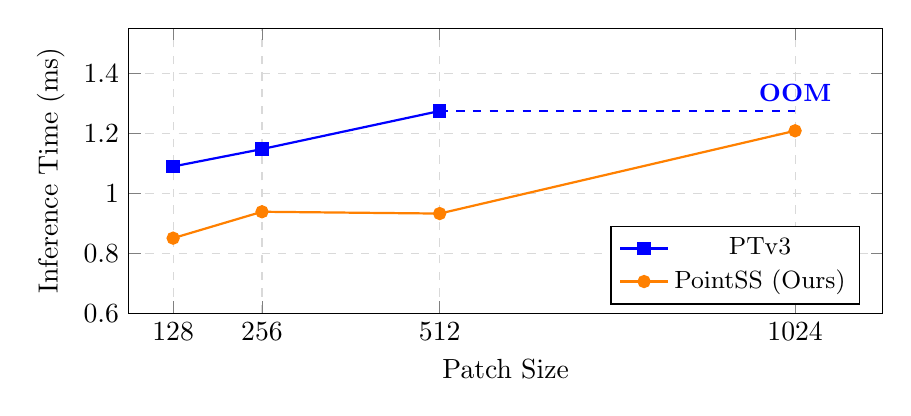
\begin{tikzpicture}
		\begin{axis}[
			width=0.92\linewidth,
			height=5.2cm,
			xlabel={Patch Size},
			ylabel={Inference Time (ms)},
			xtick={128,256,512,1024},
			xticklabels={128,256,512,1024},
			xmin=64, xmax=1150,
			ymin=0.6, ymax=1.55,
			legend pos=south east,
			legend style={font=\small},
			grid=major,
			grid style={dashed,gray!30},
			]

			\addplot[color=blue, mark=square*, thick, solid] coordinates {
				(128, 1.089)
				(256, 1.147)
				(512, 1.274)
			};
			\addlegendentry{PTv3}

			\addplot[color=orange, mark=*, thick, solid] coordinates {
				(128,  0.850)
				(256,  0.938)
				(512,  0.932)
				(1024, 1.208)
			};
			\addlegendentry{PointSS (Ours)}

			\draw[color=blue, dashed, thick] (axis cs:512,1.274) -- (axis cs:1024,1.274);
			\node[color=blue, font=\small\bfseries, anchor=south] at (axis cs:1024,1.274) {OOM};

		\end{axis}
	\end{tikzpicture}
	\caption{Inference time vs.\ patch size for PTv3 and PointSS.}
	\label{fig:efficiency}
\end{figure}

To validate the computational advantage of linear SSM complexity, we compare the inference time of PointSS against PTv3 under identical conditions: FP32 precision, batch size 1, on an NVIDIA A6000 GPU. As shown in \cref{fig:efficiency}, PointSS consistently reduces inference time by approximately 9--19\% across patch sizes from 128 to 512. At patch size 1024, PTv3 encounters out-of-memory errors due to the quadratic memory cost of self-attention, while PointSS continues to operate without constraint, demonstrating that linear complexity provides meaningful scalability advantages in large-patch-size regimes. Regarding other SSM-based methods, all approaches maintain O(N) linear complexity. While GGAM introduces additional computational cost for geometric prior extraction, this overhead is offset by accuracy gains: PointSS achieves 73.8\% mIoU compared to PCM's 69.8\% (+4.0\%) and Pamba's 73.5\% (+0.3\%), demonstrating a favorable accuracy-efficiency trade-off within the SSM family.

\subsection{Ablation Study}

Ablation studies were conducted on the S3DIS dataset using a progressive strategy to verify individual module contributions. First, the effectiveness of GGAM in mitigating the loss of spatial proximity was examined (\Cref{tab:ggam_fragmentation,tab:ggam_category,tab:ggam_components}), followed by the validation of ASD-SSM design choices (\Cref{tab:scale_constraint,tab:param_comparison,tab:scale_config}).

The baseline model utilizes a standard single-scale bidirectional Mamba. As shown in \Cref{tab:progressive_improvement}, introducing GGAM alone yields a +1.6\% mIoU improvement, confirming that extracting geometric priors through windowed neighborhoods and dual-serialization effectively mitigates serialization-induced spatial proximity loss. Building on this, ASD-SSM contributes a further +1.9\%, demonstrating that scale-decoupled parameterization is crucial for simultaneously capturing local details and modeling global semantics. Together, the two modules address distinct limitations and yield a gain of 3.5\% mIoU over the baseline.

\begin{table*}[!t]
	\centering
	\caption{Incremental performance improvement on the S3DIS dataset}
	\label{tab:progressive_improvement}
	\begin{tabular}{lll}
		\toprule
		\textbf{Model Configuration} & \textbf{mIoU (\%)} & \textbf{Improvement (\%)} \\
		\midrule
		Pure Mamba Baseline & 70.3 & - \\
		Baseline + GGAM & 71.9 & +1.6 \\
		Baseline + GGAM + ASD-SSM (PointSS) & \textbf{73.8} & +1.9 \\
		\midrule
		\textbf{Total Improvement} & - & \textbf{+3.5} \\
		\bottomrule
	\end{tabular}
\end{table*}

\begin{table*}[!t]
	\centering
	\caption{Stratified Analysis of GGAM Effectiveness by Proximity Loss Level}
	\label{tab:ggam_fragmentation}
	\begin{tabular}{llllll}
		\toprule
		\textbf{Proximity Loss} & \textbf{Point} & \textbf{Point} & \textbf{Baseline} & \textbf{GGAM} & \textbf{Absolute} \\
		\textbf{Ratio} & \textbf{Count} & \textbf{Percentage} & \textbf{IoU (\%)} & \textbf{IoU (\%)} & \textbf{Gain (\%)} \\
		\midrule
		0-10\% (Low) & 270k & 67\% & 73.0 & 73.7 & 0.7 \\
		10-20\% (Mild) & 101k & 25\% & 65.9 & 68.6 & 2.7 \\
		20-30\% (Moderate) & 32k & 8\% & 62.0 & 67.4 & 5.4 \\
		\midrule
		Total & 403k & 100\% & 70.3 & 71.9 & 1.6 \\
		\bottomrule
	\end{tabular}
	\par\vspace{3pt}
	\footnotesize Note: The proximity loss ratio is defined as the proportion of a point's K-nearest spatial neighbors that are more than 300 sequence positions away from the center point in the serialized sequence.
\end{table*}
\subsubsection{Ablation Study of GGAM}

We verify the effectiveness of GGAM through three experiments on the S3DIS dataset.

To measure the degree of spatial proximity loss for each point after serialization, we treat it as the center point and search for its 128 spatial neighbors, then compute the proportion of these neighbors that are more than 300 sequence positions away from the center point in the serialized sequence. The threshold of 300, larger than the window size (64), provides a broader sampling range for a more stable estimation of proximity loss. We term this per-point measure the \textit{proximity loss ratio}; a higher ratio indicates more severe spatial proximity loss in a point's local neighborhood. We use it to group points by their degree of spatial proximity loss and compare segmentation performance between the baseline and GGAM (\Cref{tab:ggam_fragmentation}).

Experimental results indicate that approximately 33\% of points suffer from the loss of spatial proximity under Hilbert serialization. As the proximity loss ratio increases from 0--10\% to 20--30\%, baseline performance drops sharply, confirming the impact of serialization on local geometric representation. GGAM effectively mitigates this degradation. Notably, substantial gains are observed in the high-ratio group (20--30\%), significantly exceeding improvements in the low-ratio group.



Category-wise analysis (\Cref{tab:ggam_category}) further reveals the geometric mechanism behind GGAM's effectiveness. The proximity loss ratio is distributed fairly uniformly across categories—serialization disrupts spatial neighborhoods regardless of surface type. However, the impact of this disruption varies substantially with geometric complexity. For large planar structures (e.g., floor, wall, ceiling), locally disrupted neighborhoods still convey consistent geometric context, so proximity loss has limited practical effect and GGAM provides only marginal gains. In contrast, categories with complex boundaries or irregular structures (e.g., window, door, board, clutter) are more sensitive to disrupted spatial neighbors: even a small number of misplaced neighbors can degrade local geometry estimation at edges and junctions. GGAM's explicit geometric prior injection is precisely targeted at these high-sensitivity regions, resulting in substantially larger improvements.

\begin{table*}[!t]
	\centering
	\caption{Category-wise Performance Analysis of GGAM on the S3DIS Dataset}
	\label{tab:ggam_category}
	\begin{tabular}{llll}
		\toprule
		\textbf{Category} & \textbf{Baseline IoU (\%)} & \textbf{GGAM IoU (\%)} & \textbf{Absolute Gain (\%)} \\
		\midrule
		Floor     & 97.3  & 97.5  & +0.2 \\
		Wall      & 84.4  & 84.8  & +0.4 \\
		Ceiling   & 89.9  & 90.3  & +0.4 \\
		Table     & 80.8  & 81.5  & +0.7 \\
		Bookshelf & 78.5  & 80.0  & +1.5 \\
		Chair     & 91.1  & 91.6  & +0.5 \\
		Sofa      & 81.5  & 84.3  & +2.8 \\
		Board     & 84.8  & 86.9  & +2.1 \\
		Door      & 77.6  & 80.6  & +3.0 \\
		Column    & 33.6  & 35.4  & +1.8 \\
		Window    & 58.9  & 62.4  & +3.5 \\
		Clutter   & 56.1  & 59.4  & +3.3 \\
		Beam      & 0.0   & 0.0   & 0.0   \\
		\midrule
		Mean      & 70.3  & 71.9  & +1.6 \\
		\bottomrule
	\end{tabular}
	\par\vspace{3pt}
	\footnotesize Note: The beam category is excluded from analysis, as beam instances are extremely sparse in S3DIS Area 5, yielding near-zero recall for both models.
\end{table*}

We further ablate the components of GGAM (\Cref{tab:ggam_components}) to verify their individual contributions.
Introducing dual-serialization alone leads to a slight performance drop, as different serialization methods introduce complementary but potentially conflicting neighborhood biases without an effective fusion strategy to reconcile them. Adding cross-sequence attention further yields a marked improvement, demonstrating that cross-sequence interaction plays a role in aligning complementary geometric information across different serialization patterns. Incorporating the gated fusion mechanism further refines the fused representation by adaptively balancing contributions from the two serialization branches. Adding the geometric consistency gate yields a further gain, as it derives a scalar gate from both streams to modulate the fused output, mitigating cross-stream inconsistencies.

The full combination demonstrates that these components function as a coherent whole to mitigate serialization-induced spatial proximity loss.

\begin{table}[!t]
	\centering
	\caption{Component-wise Ablation Study of the GGAM on the S3DIS Dataset}
	\label{tab:ggam_components}
	\begin{tabular}{ccccc}
		\toprule
		\textbf{DS} & \textbf{CSA} & \textbf{GFM} & \textbf{$L_{geo}$} & \textbf{mIoU (\%)} \\
		\midrule
		$\times$ & $\times$ & $\times$ & $\times$ & 70.8 \\
		\checkmark & $\times$ & $\times$ & $\times$ & 70.6 \\
		\checkmark & \checkmark & $\times$ & $\times$ & 71.2 \\
		\checkmark & \checkmark & \checkmark & $\times$ & 71.4 \\
		\checkmark & \checkmark & \checkmark & \checkmark & 71.9 \\
		\bottomrule
	\end{tabular}
	\par\vspace{3pt}
	\footnotesize Notes: DS: Dual-Serialization; CSA: Cross-Sequence Attention; GFM: Gated Fusion Mechanism; $L_{geo}$: Geometric Consistency Constraint (Gate Module). All configurations retain geometric feature extraction as it is a prerequisite of GGAM. The baseline (70.8\%) differs from the pure Mamba baseline in \Cref{tab:progressive_improvement} (70.3\%), as geometric feature extraction is retained in all configurations here.
\end{table}

\subsubsection{ASD-SSM Ablation Study}

We conduct systematic ablation experiments on S3DIS to evaluate key ASD-SSM design choices.

We first analyze the role of the scale constraint factor $\alpha_s$ in controlling the value range of $\bar{A}_s$. Smaller $\alpha_s$ values constrain $\bar{A}_s$ to a low range, inducing rapid state decay that enables the capture of local geometric detail, whereas larger values allow slow decay, supporting the modeling of long-range dependencies and global semantic context (\Cref{tab:scale_constraint}).
Experimental results indicate that uniform $\alpha_s$ configurations consistently underperform relative to non-uniform configurations, confirming that distinct scales require scale-specific state-decay characteristics. The best performance among the tested configurations is achieved when $\alpha_s$ increases progressively from fine to coarse scales (0.3, 0.6, 0.9). This validates the design philosophy: fine scales benefit from rapid decay to capture local geometric detail, while coarse scales require slow decay to maintain long-range state memory. Reversing this configuration leads to a notable performance drop, as excessively long state retention at fine scales interferes with local geometric modeling, while rapid decay at coarse scales disrupts the capture of global semantic context.

\begin{table}[!t]
	\centering
	\caption{Ablation Study of Scale Constraint Factors $\alpha_s$ with a 3-Scale Configuration. Results are the median of three independent runs.}
	\label{tab:scale_constraint}
	\begin{tabular}{cccc}
		\toprule
		$\alpha_1$ & $\alpha_2$ & $\alpha_3$ & \textbf{mIoU (\%)} \\
		\midrule
		0.3 & 0.3 & 0.3 & 72.3 \\
		0.7 & 0.7 & 0.7 & 72.1 \\
		0.5 & 0.5 & 0.5 & 72.6 \\
		0.3 & 0.5 & 0.7 & 73.3 \\
		0.3 & 0.6 & 0.9 & 73.8 \\
		0.3 & 0.7 & 0.9 & 73.6 \\
		0.2 & 0.6 & 0.9 & 73.2 \\
		0.4 & 0.6 & 0.9 & 73.3 \\
		0.9 & 0.6 & 0.3 & 66.5 \\
		\bottomrule
	\end{tabular}
\end{table}

We further compare ASD-SSM against several common parameterization strategies, as summarized in \Cref{tab:param_comparison}. The Shared Parameter scheme---in which all three scales share a single $\bar{A}$ matrix---treats all scales identically, failing to adapt to their distinct modeling requirements, yielding the lowest performance. The Independent Parameters scheme assigns a dedicated  $\bar{A}_s$ to each scale, capturing scale-specific characteristics but remaining input-invariant within each scale. The Parameter Interpolation approach generates $\bar{A}_s$ dynamically for the finest and coarsest scales via the parameter generator, while intermediate scales obtain their $\bar{A}_s$ through linear interpolation between $\bar{A}_1$ and $\bar{A}_S$; yet, linear interpolation fails to capture non-linear cross-scale relationships, resulting in limited gains. In contrast, ASD-SSM outperforms the Independent Parameters scheme, demonstrating that dynamic scale-aware parameter generation is a more effective parameterization strategy than static per-scale assignment.

\begin{table}[!t]
	\centering
	\caption{Performance Comparison of Different Parameterization Methods}
	\label{tab:param_comparison}
	\begin{tabular}{ll}
		\toprule
		\textbf{Parameterization Method} & \textbf{mIoU (\%)} \\
		\midrule
		Shared Parameters & 70.8 \\
		Independent Parameters & 71.6 \\
		Parameter Interpolation & 71.5 \\
		ASD-SSM (Ours) & 73.8 \\
		\bottomrule
	\end{tabular}
\end{table}

We systematically investigate the number of scales $S$ and window expansion configurations (\Cref{tab:scale_config}), confirming the necessity of hierarchical multi-scale modeling. Introducing a second scale consistently improves over the single-scale baseline, with the best 2-scale result reaching 72.4\%. Incorporating a third scale yields a further improvement, with the best 3-scale configuration achieving 73.8\%. This suggests that a three-level hierarchy---local, intermediate, and global---provides comprehensive structural representation.

Regarding window size expansion, moderate increases in the expansion factor enhance context modeling, whereas excessively large windows tend to wash out local geometric detail. Although a four-scale configuration yields a marginal additional gain of 0.2\%, it incurs longer training time with diminishing returns. Consequently, the three-scale configuration with expansion factors $(1, 2, 4)$ represents the optimal trade-off between performance and efficiency.

\begin{table}[!t]
	\centering
	\caption{Detailed Ablation Study of Scale Quantities and Window Configurations}
	\label{tab:scale_config}
	\begin{tabular}{llll}
		\toprule
		\textbf{S} & \textbf{F} & \textbf{Train Time} & \textbf{mIoU (\%)} \\
		\midrule
		1 & (1) & 35h & 71.9 \\
		2 & (1,2) & 39h & 72.1 \\
		2 & (1,3) & 40h & 72.4 \\
		2 & (1,4) & 40h & 71.7 \\
		3 & (1,2,2) & 45h & 73.6 \\
		3 & (1,2,3) & 46h & 73.6 \\
		3 & (1,2,4) & 46h & 73.8 \\
		3 & (1,3,3) & 45h & 73.4 \\
		4 & (1,2,2,2) & 53h & 73.8 \\
		4 & (1,2,2,3) & 54h & 74.0 \\
		\bottomrule
	\end{tabular}
	\par\vspace{3pt}
	\footnotesize Notes: S: Number of scales; F: Scaling factors for window expansion; Train Time: Total training duration on the S3DIS dataset.
\end{table}

\subsection{Qualitative Experiment}

\cref{fig:vis} presents a comparison of segmentation results among PointSS, Point Transformer, and Point Cloud Mamba across four scenes on the S3DIS dataset. As highlighted by the circles in the figure, PointSS demonstrates advantages in the following three types of regions.

For structures with large spatial spans such as windows (upper circle in office\_10), baseline methods produce noticeably fragmented or incomplete predictions; PointSS, by contrast, yields more complete segmentation regions with higher agreement with the ground truth. This improvement is attributed to GGAM's explicit modeling of geometric relationships within windowed neighborhoods, which compensates for the context discontinuity caused by the loss of spatial proximity during serialization.

In regions comprising small, irregular objects such as clutter (lower circle in office\_12 and office\_14), baseline methods tend to confuse these regions with surrounding tables and chairs, resulting in unstable boundary predictions. PointSS leverages the rapid state decay at fine-grained scales within its multi-scale architecture to respond more effectively to local geometric variations, yielding more accurate category predictions in such regions.

At category boundaries such as those between bookcase and wall (office\_13), baseline methods exhibit blurred or misclassified predictions, whereas PointSS produces sharper and more accurate boundaries. Through slow state decay, ASD-SSM's coarse-grained scales retain broader contextual information, thereby improving boundary prediction consistency.

These qualitative results are consistent with the trends observed in the quantitative experiments, further validating the effectiveness of PointSS in complex indoor scenes.

\begin{figure*}[!t]
	\centering
	\includegraphics[width=\textwidth]{picture/visualize.JPG}
	\caption{Qualitative comparison of semantic segmentation results on four representative indoor scenes (Area 5 of S3DIS).}
	\label{fig:vis}
\end{figure*}

\section{Conclusion}

This paper presents PointSS, a geometry-aware multi-scale framework for point cloud analysis built upon State Space Models. GGAM and ASD-SSM address the two key limitations of existing SSM-based methods—serialization-induced spatial proximity loss and input-invariant state transition parameters—respectively. Experiments on S3DIS and ModelNet40 demonstrate strong segmentation performance and competitive classification accuracy, consistently outperforming major SSM-based counterparts.

Despite these contributions, PointSS has several limitations. The scale constraint factors $\alpha_s$ are manually specified as fixed hyperparameters, which may require task-specific tuning when generalizing to new datasets or point cloud distributions. In addition, the dual-serialization design in GGAM introduces additional computational overhead compared to single-stream methods. Furthermore, PointSS has only been evaluated on indoor scene segmentation and synthetic object classification benchmarks; its effectiveness on outdoor LiDAR datasets (e.g., SemanticKITTI) remains to be verified.

Future work will explore automatically learning the scale constraint factors to reduce the need for manual tuning. Extending PointSS to large-scale outdoor datasets and investigating more efficient geometric feature fusion strategies are also directions we intend to pursue.

\section*{Acknowledgment}
This paper is funded by 20260301004YY.

\bibliographystyle{cas-model2-names}
\bibliography{../IEEE-Transactions-LaTeX2e-templates-and-instructions/ref}

\end{document}

